\documentclass[twoside]{book}

% Packages required by doxygen
\usepackage{fixltx2e}
\usepackage{calc}
\usepackage{doxygen}
\usepackage[export]{adjustbox} % also loads graphicx
\usepackage{graphicx}
\usepackage[utf8]{inputenc}
\usepackage{makeidx}
\usepackage{multicol}
\usepackage{multirow}
\PassOptionsToPackage{warn}{textcomp}
\usepackage{textcomp}
\usepackage[nointegrals]{wasysym}
\usepackage[table]{xcolor}

% Font selection
\usepackage[T1]{fontenc}
\usepackage[scaled=.90]{helvet}
\usepackage{courier}
\usepackage{amssymb}
\usepackage{sectsty}
\renewcommand{\familydefault}{\sfdefault}
\allsectionsfont{%
  \fontseries{bc}\selectfont%
  \color{darkgray}%
}
\renewcommand{\DoxyLabelFont}{%
  \fontseries{bc}\selectfont%
  \color{darkgray}%
}
\newcommand{\+}{\discretionary{\mbox{\scriptsize$\hookleftarrow$}}{}{}}

% Page & text layout
\usepackage{geometry}
\geometry{%
  a4paper,%
  top=2.5cm,%
  bottom=2.5cm,%
  left=2.5cm,%
  right=2.5cm%
}
\tolerance=750
\hfuzz=15pt
\hbadness=750
\setlength{\emergencystretch}{15pt}
\setlength{\parindent}{0cm}
\setlength{\parskip}{3ex plus 2ex minus 2ex}
\makeatletter
\renewcommand{\paragraph}{%
  \@startsection{paragraph}{4}{0ex}{-1.0ex}{1.0ex}{%
    \normalfont\normalsize\bfseries\SS@parafont%
  }%
}
\renewcommand{\subparagraph}{%
  \@startsection{subparagraph}{5}{0ex}{-1.0ex}{1.0ex}{%
    \normalfont\normalsize\bfseries\SS@subparafont%
  }%
}
\makeatother

% Headers & footers
\usepackage{fancyhdr}
\pagestyle{fancyplain}
\fancyhead[LE]{\fancyplain{}{\bfseries\thepage}}
\fancyhead[CE]{\fancyplain{}{}}
\fancyhead[RE]{\fancyplain{}{\bfseries\leftmark}}
\fancyhead[LO]{\fancyplain{}{\bfseries\rightmark}}
\fancyhead[CO]{\fancyplain{}{}}
\fancyhead[RO]{\fancyplain{}{\bfseries\thepage}}
\fancyfoot[LE]{\fancyplain{}{}}
\fancyfoot[CE]{\fancyplain{}{}}
\fancyfoot[RE]{\fancyplain{}{\bfseries\scriptsize Generated by Doxygen }}
\fancyfoot[LO]{\fancyplain{}{\bfseries\scriptsize Generated by Doxygen }}
\fancyfoot[CO]{\fancyplain{}{}}
\fancyfoot[RO]{\fancyplain{}{}}
\renewcommand{\footrulewidth}{0.4pt}
\renewcommand{\chaptermark}[1]{%
  \markboth{#1}{}%
}
\renewcommand{\sectionmark}[1]{%
  \markright{\thesection\ #1}%
}

% Indices & bibliography
\usepackage{natbib}
\usepackage[titles]{tocloft}
\setcounter{tocdepth}{3}
\setcounter{secnumdepth}{5}
\makeindex

% Hyperlinks (required, but should be loaded last)
\usepackage{ifpdf}
\ifpdf
  \usepackage[pdftex,pagebackref=true]{hyperref}
\else
  \usepackage[ps2pdf,pagebackref=true]{hyperref}
\fi
\hypersetup{%
  colorlinks=true,%
  linkcolor=blue,%
  citecolor=blue,%
  unicode%
}

% Custom commands
\newcommand{\clearemptydoublepage}{%
  \newpage{\pagestyle{empty}\cleardoublepage}%
}

\usepackage{caption}
\captionsetup{labelsep=space,justification=centering,font={bf},singlelinecheck=off,skip=4pt,position=top}

%===== C O N T E N T S =====

\begin{document}

% Titlepage & ToC
\hypersetup{pageanchor=false,
             bookmarksnumbered=true,
             pdfencoding=unicode
            }
\pagenumbering{alph}
\begin{titlepage}
\vspace*{7cm}
\begin{center}%
{\Large Grafos \\[1ex]\large 1 }\\
\vspace*{1cm}
{\large Generated by Doxygen 1.8.13}\\
\end{center}
\end{titlepage}
\clearemptydoublepage
\pagenumbering{roman}
\tableofcontents
\clearemptydoublepage
\pagenumbering{arabic}
\hypersetup{pageanchor=true}

%--- Begin generated contents ---
\chapter{Class Index}
\section{Class List}
Here are the classes, structs, unions and interfaces with brief descriptions\+:\begin{DoxyCompactList}
\item\contentsline{section}{\hyperlink{class_binary_search_tree}{Binary\+Search\+Tree$<$ Data, Type\+Nodo $>$} }{\pageref{class_binary_search_tree}}{}
\item\contentsline{section}{\hyperlink{class_circulo}{Circulo} \\*Clase que se encarga e modelar un circulo }{\pageref{class_circulo}}{}
\item\contentsline{section}{\hyperlink{class_class_node}{Class\+Node$<$ Dato $>$} }{\pageref{class_class_node}}{}
\item\contentsline{section}{\hyperlink{class_dato_no_primitivo}{Dato\+No\+Primitivo$<$ Tipo\+Dato $>$} }{\pageref{class_dato_no_primitivo}}{}
\item\contentsline{section}{\hyperlink{class_equilatero}{Equilatero} \\*Calse equilatero }{\pageref{class_equilatero}}{}
\item\contentsline{section}{\hyperlink{class_escaleno}{Escaleno} \\*Calse \hyperlink{class_escaleno}{Escaleno} }{\pageref{class_escaleno}}{}
\item\contentsline{section}{\hyperlink{class_figura}{Figura} \\*Clase que se encarga de crear una figura en 2D }{\pageref{class_figura}}{}
\item\contentsline{section}{\hyperlink{class_impresora}{Impresora$<$ T $>$} \\*Clase que imprmime objetos }{\pageref{class_impresora}}{}
\item\contentsline{section}{\hyperlink{class_isosceles}{Isosceles} \\*Calse \hyperlink{class_isosceles}{Isosceles} }{\pageref{class_isosceles}}{}
\item\contentsline{section}{\hyperlink{class_principal}{Principal} }{\pageref{class_principal}}{}
\item\contentsline{section}{\hyperlink{classrectangulo}{rectangulo} \\*Clase rectangulo }{\pageref{classrectangulo}}{}
\item\contentsline{section}{\hyperlink{classtriangulo}{triangulo} \\*Calse tringulo }{\pageref{classtriangulo}}{}
\item\contentsline{section}{\hyperlink{class_vertice}{Vertice} \\*Clase que modela un punto en el espacio }{\pageref{class_vertice}}{}
\end{DoxyCompactList}

\chapter{Class Documentation}
\hypertarget{class_binary_search_tree}{}\section{Binary\+Search\+Tree$<$ Data, Type\+Nodo $>$ Class Template Reference}
\label{class_binary_search_tree}\index{Binary\+Search\+Tree$<$ Data, Type\+Nodo $>$@{Binary\+Search\+Tree$<$ Data, Type\+Nodo $>$}}


Collaboration diagram for Binary\+Search\+Tree$<$ Data, Type\+Nodo $>$\+:
\nopagebreak
\begin{figure}[H]
\begin{center}
\leavevmode
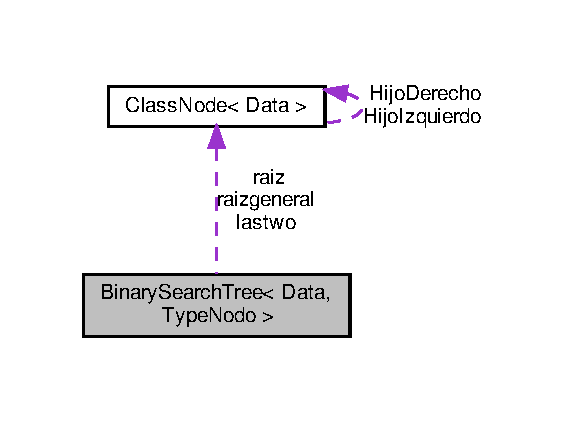
\includegraphics[width=272pt]{class_binary_search_tree__coll__graph}
\end{center}
\end{figure}
\subsection*{Public Member Functions}
\begin{DoxyCompactItemize}
\item 
\mbox{\Hypertarget{class_binary_search_tree_adfac6a810d0b81e6772c63808684c8b2}\label{class_binary_search_tree_adfac6a810d0b81e6772c63808684c8b2}} 
Type\+Nodo \& {\bfseries insert} (const Data \&dato)
\item 
\mbox{\Hypertarget{class_binary_search_tree_af1b0c6778ed2f1a57d598ef33358b6d9}\label{class_binary_search_tree_af1b0c6778ed2f1a57d598ef33358b6d9}} 
Type\+Nodo $\ast$ \hyperlink{class_binary_search_tree_af1b0c6778ed2f1a57d598ef33358b6d9}{larges\+To\+The\+Left} (Type\+Nodo \&nodo\+Inicial)
\begin{DoxyCompactList}\small\item\em Funcion que devuelve el hijo mas grande a la izquierda. \end{DoxyCompactList}\item 
\mbox{\Hypertarget{class_binary_search_tree_a0f845aaaa83043d56c187117e5829b9b}\label{class_binary_search_tree_a0f845aaaa83043d56c187117e5829b9b}} 
Type\+Nodo $\ast$ \hyperlink{class_binary_search_tree_a0f845aaaa83043d56c187117e5829b9b}{smalles\+To\+The\+Right} (Type\+Nodo \&nodo\+Inicial)
\begin{DoxyCompactList}\small\item\em Funcion que devuelve el hijo mas pequeño a la derecha. \end{DoxyCompactList}\item 
\mbox{\Hypertarget{class_binary_search_tree_a2267a608fb78e1eafe4531a67d2bf7c8}\label{class_binary_search_tree_a2267a608fb78e1eafe4531a67d2bf7c8}} 
Type\+Nodo $\ast$ \hyperlink{class_binary_search_tree_a2267a608fb78e1eafe4531a67d2bf7c8}{Node\+Of} (Data \&el\+Dato)
\begin{DoxyCompactList}\small\item\em funcion que devuelve el nodo de un dato \end{DoxyCompactList}\item 
\mbox{\Hypertarget{class_binary_search_tree_ac08a812f7c83c1ee9a274099b38b5a62}\label{class_binary_search_tree_ac08a812f7c83c1ee9a274099b38b5a62}} 
Data $\ast$ \hyperlink{class_binary_search_tree_ac08a812f7c83c1ee9a274099b38b5a62}{data\+In} (Type\+Nodo \&el\+Nodo)
\begin{DoxyCompactList}\small\item\em funcion que devuelve el dato de un nodo \end{DoxyCompactList}\item 
\mbox{\Hypertarget{class_binary_search_tree_a00b5c4aef3fae5ec348363e29e8b5cbf}\label{class_binary_search_tree_a00b5c4aef3fae5ec348363e29e8b5cbf}} 
void \hyperlink{class_binary_search_tree_a00b5c4aef3fae5ec348363e29e8b5cbf}{remove} (Data \&dato\+A\+Borrar)
\begin{DoxyCompactList}\small\item\em funcion que borra el nodo de un arbol \end{DoxyCompactList}\item 
\mbox{\Hypertarget{class_binary_search_tree_a6c83485425575c196701ca5e28d7f0e6}\label{class_binary_search_tree_a6c83485425575c196701ca5e28d7f0e6}} 
int \hyperlink{class_binary_search_tree_a6c83485425575c196701ca5e28d7f0e6}{Existe} (Data \&el\+Dato)
\begin{DoxyCompactList}\small\item\em funcion que devuelve si el dato existe o no return bandera 1 si existe 0 si no \end{DoxyCompactList}\item 
\mbox{\Hypertarget{class_binary_search_tree_ad1ef774f107b357863b1b578d0723553}\label{class_binary_search_tree_ad1ef774f107b357863b1b578d0723553}} 
void {\bfseries preorden} (\hyperlink{class_class_node}{Class\+Node}$<$ Data $>$ $\ast$n)
\item 
\mbox{\Hypertarget{class_binary_search_tree_a957d1cd0c14f897c4847753ce82a41d7}\label{class_binary_search_tree_a957d1cd0c14f897c4847753ce82a41d7}} 
void {\bfseries In\+Orden} (\hyperlink{class_class_node}{Class\+Node}$<$ Data $>$ $\ast$n)
\item 
\mbox{\Hypertarget{class_binary_search_tree_a2119d18706ac114900c67d828c7ad476}\label{class_binary_search_tree_a2119d18706ac114900c67d828c7ad476}} 
void {\bfseries Post\+Orden} (\hyperlink{class_class_node}{Class\+Node}$<$ Data $>$ $\ast$n)
\item 
int \hyperlink{class_binary_search_tree_a922ad2464f2085d208847a76fca1bb51}{calcular\+Niveles} (\hyperlink{class_class_node}{Class\+Node}$<$ Data $>$ $\ast$inicio)
\begin{DoxyCompactList}\small\item\em funcion recursiva que calcula la cantidad de niveles a partir de un nodo \end{DoxyCompactList}\item 
int \hyperlink{class_binary_search_tree_adb25fc678a13dbaa05ba0c0627eb232e}{calcular\+Nodos} (\hyperlink{class_class_node}{Class\+Node}$<$ Data $>$ $\ast$inicio, int nivel)
\begin{DoxyCompactList}\small\item\em funcion recursiva que calcula la cantidad de nodos en un nivel \end{DoxyCompactList}\item 
string \hyperlink{class_binary_search_tree_a30a79ed298da4d6fe4395dddd53842b8}{devolver\+String\+Nivel} (\hyperlink{class_class_node}{Class\+Node}$<$ Data $>$ $\ast$inicio, int nivel, int cantidad\+Datos)
\begin{DoxyCompactList}\small\item\em funcion recursiva que devuelve la representacion de texto de un nivel \end{DoxyCompactList}\item 
\mbox{\Hypertarget{class_binary_search_tree_af6e24d171e86e3c3a9092dbb822e4411}\label{class_binary_search_tree_af6e24d171e86e3c3a9092dbb822e4411}} 
void \hyperlink{class_binary_search_tree_af6e24d171e86e3c3a9092dbb822e4411}{print} ()
\begin{DoxyCompactList}\small\item\em funcion que imprime un arbol \end{DoxyCompactList}\item 
\mbox{\Hypertarget{class_binary_search_tree_ad1ef774f107b357863b1b578d0723553}\label{class_binary_search_tree_ad1ef774f107b357863b1b578d0723553}} 
void {\bfseries preorden} (\hyperlink{class_class_node}{Class\+Node}$<$ Data $>$ $\ast$n)
\end{DoxyCompactItemize}
\subsection*{Public Attributes}
\begin{DoxyCompactItemize}
\item 
\mbox{\Hypertarget{class_binary_search_tree_a03b6a961580af63ef22085b6f421c639}\label{class_binary_search_tree_a03b6a961580af63ef22085b6f421c639}} 
\hyperlink{class_class_node}{Class\+Node}$<$ Data $>$ $\ast$ {\bfseries lastwo}
\item 
\mbox{\Hypertarget{class_binary_search_tree_a16ae9eac3a2653c15ec2bfb64172f8d0}\label{class_binary_search_tree_a16ae9eac3a2653c15ec2bfb64172f8d0}} 
\hyperlink{class_class_node}{Class\+Node}$<$ Data $>$ $\ast$ {\bfseries raizgeneral}
\item 
\mbox{\Hypertarget{class_binary_search_tree_a15180798e7105d7ec936e5741628c156}\label{class_binary_search_tree_a15180798e7105d7ec936e5741628c156}} 
\hyperlink{class_class_node}{Class\+Node}$<$ Data $>$ $\ast$ {\bfseries raiz}
\item 
\mbox{\Hypertarget{class_binary_search_tree_a187988de7db6639f0541d59ef27e8ab6}\label{class_binary_search_tree_a187988de7db6639f0541d59ef27e8ab6}} 
int {\bfseries items} =0
\end{DoxyCompactItemize}


\subsection{Detailed Description}
\subsubsection*{template$<$typename Data, typename Type\+Nodo$>$\newline
class Binary\+Search\+Tree$<$ Data, Type\+Nodo $>$}



Definition at line 10 of file Binary\+Search\+Tree.\+h.



\subsection{Member Function Documentation}
\mbox{\Hypertarget{class_binary_search_tree_a922ad2464f2085d208847a76fca1bb51}\label{class_binary_search_tree_a922ad2464f2085d208847a76fca1bb51}} 
\index{Binary\+Search\+Tree@{Binary\+Search\+Tree}!calcular\+Niveles@{calcular\+Niveles}}
\index{calcular\+Niveles@{calcular\+Niveles}!Binary\+Search\+Tree@{Binary\+Search\+Tree}}
\subsubsection{\texorpdfstring{calcular\+Niveles()}{calcularNiveles()}}
{\footnotesize\ttfamily template$<$typename Data, typename Type\+Nodo$>$ \\
int \hyperlink{class_binary_search_tree}{Binary\+Search\+Tree}$<$ Data, Type\+Nodo $>$\+::calcular\+Niveles (\begin{DoxyParamCaption}\item[{\hyperlink{class_class_node}{Class\+Node}$<$ Data $>$ $\ast$}]{inicio }\end{DoxyParamCaption})\hspace{0.3cm}{\ttfamily [inline]}}



funcion recursiva que calcula la cantidad de niveles a partir de un nodo 


\begin{DoxyParams}{Parameters}
{\em inicio} & es un puntero a la direccion de memoria \\
\hline
\end{DoxyParams}


Definition at line 497 of file Binary\+Search\+Tree.\+h.

\mbox{\Hypertarget{class_binary_search_tree_adb25fc678a13dbaa05ba0c0627eb232e}\label{class_binary_search_tree_adb25fc678a13dbaa05ba0c0627eb232e}} 
\index{Binary\+Search\+Tree@{Binary\+Search\+Tree}!calcular\+Nodos@{calcular\+Nodos}}
\index{calcular\+Nodos@{calcular\+Nodos}!Binary\+Search\+Tree@{Binary\+Search\+Tree}}
\subsubsection{\texorpdfstring{calcular\+Nodos()}{calcularNodos()}}
{\footnotesize\ttfamily template$<$typename Data, typename Type\+Nodo$>$ \\
int \hyperlink{class_binary_search_tree}{Binary\+Search\+Tree}$<$ Data, Type\+Nodo $>$\+::calcular\+Nodos (\begin{DoxyParamCaption}\item[{\hyperlink{class_class_node}{Class\+Node}$<$ Data $>$ $\ast$}]{inicio,  }\item[{int}]{nivel }\end{DoxyParamCaption})\hspace{0.3cm}{\ttfamily [inline]}}



funcion recursiva que calcula la cantidad de nodos en un nivel 


\begin{DoxyParams}{Parameters}
{\em inicio} & es un puntero a la direccion de memoria \\
\hline
{\em nivel} & es el nivel que se quiere \\
\hline
\end{DoxyParams}


Definition at line 548 of file Binary\+Search\+Tree.\+h.

\mbox{\Hypertarget{class_binary_search_tree_a30a79ed298da4d6fe4395dddd53842b8}\label{class_binary_search_tree_a30a79ed298da4d6fe4395dddd53842b8}} 
\index{Binary\+Search\+Tree@{Binary\+Search\+Tree}!devolver\+String\+Nivel@{devolver\+String\+Nivel}}
\index{devolver\+String\+Nivel@{devolver\+String\+Nivel}!Binary\+Search\+Tree@{Binary\+Search\+Tree}}
\subsubsection{\texorpdfstring{devolver\+String\+Nivel()}{devolverStringNivel()}}
{\footnotesize\ttfamily template$<$typename Data, typename Type\+Nodo$>$ \\
string \hyperlink{class_binary_search_tree}{Binary\+Search\+Tree}$<$ Data, Type\+Nodo $>$\+::devolver\+String\+Nivel (\begin{DoxyParamCaption}\item[{\hyperlink{class_class_node}{Class\+Node}$<$ Data $>$ $\ast$}]{inicio,  }\item[{int}]{nivel,  }\item[{int}]{cantidad\+Datos }\end{DoxyParamCaption})\hspace{0.3cm}{\ttfamily [inline]}}



funcion recursiva que devuelve la representacion de texto de un nivel 


\begin{DoxyParams}{Parameters}
{\em inicio} & es un puntero a la direccion de memoria \\
\hline
{\em nivel} & es el nivel que se quiere \\
\hline
\end{DoxyParams}


Definition at line 590 of file Binary\+Search\+Tree.\+h.



The documentation for this class was generated from the following file\+:\begin{DoxyCompactItemize}
\item 
/home/jzunigame/\+Documentos/\+A\+\_\+\+Algoritmos/\+A\+\_\+\+Git/\+Laboratorios/\+Lab5 Arboles/include/Binary\+Search\+Tree.\+h\end{DoxyCompactItemize}

\hypertarget{class_class_arista}{}\section{Class\+Arista Class Reference}
\label{class_class_arista}\index{Class\+Arista@{Class\+Arista}}


Collaboration diagram for Class\+Arista\+:
\nopagebreak
\begin{figure}[H]
\begin{center}
\leavevmode
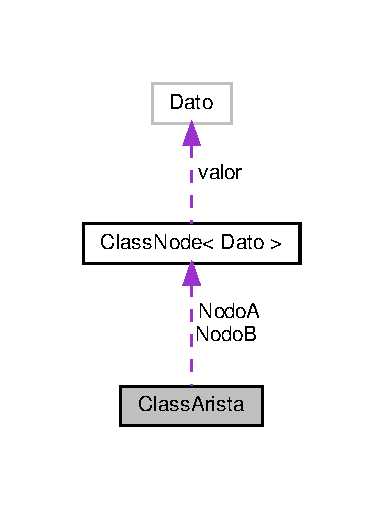
\includegraphics[width=184pt]{class_class_arista__coll__graph}
\end{center}
\end{figure}
\subsection*{Public Member Functions}
\begin{DoxyCompactItemize}
\item 
\mbox{\Hypertarget{class_class_arista_ac0fc70beb470285da7bcdfd97848aef1}\label{class_class_arista_ac0fc70beb470285da7bcdfd97848aef1}} 
{\bfseries Class\+Arista} (\hyperlink{class_class_node}{Class\+Node} $\ast$NodoA, \hyperlink{class_class_node}{Class\+Node} $\ast$NodoB, string Arista\+ID)
\item 
\mbox{\Hypertarget{class_class_arista_ac0fc70beb470285da7bcdfd97848aef1}\label{class_class_arista_ac0fc70beb470285da7bcdfd97848aef1}} 
{\bfseries Class\+Arista} (\hyperlink{class_class_node}{Class\+Node} $\ast$NodoA, \hyperlink{class_class_node}{Class\+Node} $\ast$NodoB, string Arista\+ID)
\item 
\mbox{\Hypertarget{class_class_arista_ac0fc70beb470285da7bcdfd97848aef1}\label{class_class_arista_ac0fc70beb470285da7bcdfd97848aef1}} 
{\bfseries Class\+Arista} (\hyperlink{class_class_node}{Class\+Node} $\ast$NodoA, \hyperlink{class_class_node}{Class\+Node} $\ast$NodoB, string Arista\+ID)
\item 
\mbox{\Hypertarget{class_class_arista_ac0fc70beb470285da7bcdfd97848aef1}\label{class_class_arista_ac0fc70beb470285da7bcdfd97848aef1}} 
{\bfseries Class\+Arista} (\hyperlink{class_class_node}{Class\+Node} $\ast$NodoA, \hyperlink{class_class_node}{Class\+Node} $\ast$NodoB, string Arista\+ID)
\item 
\mbox{\Hypertarget{class_class_arista_ac0fc70beb470285da7bcdfd97848aef1}\label{class_class_arista_ac0fc70beb470285da7bcdfd97848aef1}} 
{\bfseries Class\+Arista} (\hyperlink{class_class_node}{Class\+Node} $\ast$NodoA, \hyperlink{class_class_node}{Class\+Node} $\ast$NodoB, string Arista\+ID)
\item 
\mbox{\Hypertarget{class_class_arista_ac0fc70beb470285da7bcdfd97848aef1}\label{class_class_arista_ac0fc70beb470285da7bcdfd97848aef1}} 
{\bfseries Class\+Arista} (\hyperlink{class_class_node}{Class\+Node} $\ast$NodoA, \hyperlink{class_class_node}{Class\+Node} $\ast$NodoB, string Arista\+ID)
\end{DoxyCompactItemize}
\subsection*{Public Attributes}
\begin{DoxyCompactItemize}
\item 
\mbox{\Hypertarget{class_class_arista_a867b108f8dca29179c6c504eedaac73b}\label{class_class_arista_a867b108f8dca29179c6c504eedaac73b}} 
\hyperlink{class_class_node}{Class\+Node} $\ast$ {\bfseries NodoA} =0x0
\item 
\mbox{\Hypertarget{class_class_arista_af06f999774a34a959e6f08242fa6576b}\label{class_class_arista_af06f999774a34a959e6f08242fa6576b}} 
\hyperlink{class_class_node}{Class\+Node} $\ast$ {\bfseries NodoB} =0x0
\item 
\mbox{\Hypertarget{class_class_arista_a4a587b16ba639f0bf1203ab03195f02b}\label{class_class_arista_a4a587b16ba639f0bf1203ab03195f02b}} 
float {\bfseries peso}
\item 
\mbox{\Hypertarget{class_class_arista_ae5f9008070524e0b1185485c6dd9dfdf}\label{class_class_arista_ae5f9008070524e0b1185485c6dd9dfdf}} 
string {\bfseries Arista\+ID}
\item 
\mbox{\Hypertarget{class_class_arista_a8f4f028af3d4a1b96464db939dd1b86c}\label{class_class_arista_a8f4f028af3d4a1b96464db939dd1b86c}} 
string {\bfseries valor}
\end{DoxyCompactItemize}


\subsection{Detailed Description}


Definition at line 6 of file graph.\+h.



The documentation for this class was generated from the following files\+:\begin{DoxyCompactItemize}
\item 
Algoritmos\+De\+Terceros/include/graph.\+h\item 
Algoritmos\+De\+Terceros/include/graph2.\+h\item 
Algoritmos\+De\+Terceros/include/Mi\+Clase\+Arista.\+h\end{DoxyCompactItemize}

\hypertarget{class_class_node}{}\section{Class\+Node$<$ Dato $>$ Class Template Reference}
\label{class_class_node}\index{Class\+Node$<$ Dato $>$@{Class\+Node$<$ Dato $>$}}


Collaboration diagram for Class\+Node$<$ Dato $>$\+:\nopagebreak
\begin{figure}[H]
\begin{center}
\leavevmode
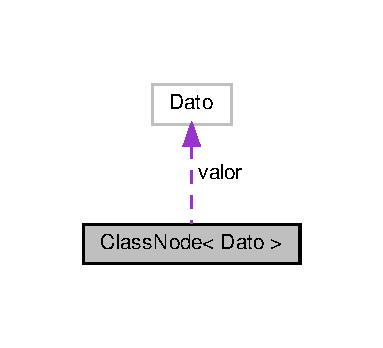
\includegraphics[width=184pt]{class_class_node__coll__graph}
\end{center}
\end{figure}
\subsection*{Public Member Functions}
\begin{DoxyCompactItemize}
\item 
\mbox{\Hypertarget{class_class_node_ac14b1ea4ba58bd16d53c2fdc0778bbda}\label{class_class_node_ac14b1ea4ba58bd16d53c2fdc0778bbda}} 
{\bfseries Class\+Node} (Dato $\ast$valor)
\end{DoxyCompactItemize}
\subsection*{Public Attributes}
\begin{DoxyCompactItemize}
\item 
\mbox{\Hypertarget{class_class_node_ac29f0086e122a3114b8130d1ba58d010}\label{class_class_node_ac29f0086e122a3114b8130d1ba58d010}} 
\hyperlink{class_class_node}{Class\+Node}$<$ Dato $>$ $\ast$ {\bfseries Hijo\+Izquierdo} = 0x0
\item 
\mbox{\Hypertarget{class_class_node_a0fbbfce087dba9ffa6d1c67bc9e0b58c}\label{class_class_node_a0fbbfce087dba9ffa6d1c67bc9e0b58c}} 
\hyperlink{class_class_node}{Class\+Node}$<$ Dato $>$ $\ast$ {\bfseries Hijo\+Derecho} = 0x0
\item 
\mbox{\Hypertarget{class_class_node_a0a597e54b607022b1486e254d8a64880}\label{class_class_node_a0a597e54b607022b1486e254d8a64880}} 
Dato $\ast$ {\bfseries valor}
\end{DoxyCompactItemize}


\subsection{Detailed Description}
\subsubsection*{template$<$typename Dato$>$\newline
class Class\+Node$<$ Dato $>$}



Definition at line 9 of file Node.\+h.



The documentation for this class was generated from the following file\+:\begin{DoxyCompactItemize}
\item 
/home/jzunigame/\+Documentos/\+A\+\_\+\+Algoritmos/\+A\+\_\+\+Git/\+Laboratorios/\+Lab5 Arboles/include/Node.\+h\end{DoxyCompactItemize}

\hypertarget{class_element}{}\section{Element$<$ D $>$ Class Template Reference}
\label{class_element}\index{Element$<$ D $>$@{Element$<$ D $>$}}
\subsection*{Public Member Functions}
\begin{DoxyCompactItemize}
\item 
\mbox{\Hypertarget{class_element_a4dff9b63467ee6287327b255396f0988}\label{class_element_a4dff9b63467ee6287327b255396f0988}} 
{\bfseries Element} (D d)
\item 
\mbox{\Hypertarget{class_element_a2a953047eeec5513b8942a02570f7ced}\label{class_element_a2a953047eeec5513b8942a02570f7ced}} 
{\bfseries Element} (const \hyperlink{class_element}{Element} \&orig)
\item 
\mbox{\Hypertarget{class_element_a346f8fee69720a230e3374c844d18f3e}\label{class_element_a346f8fee69720a230e3374c844d18f3e}} 
D {\bfseries get} ()
\item 
\mbox{\Hypertarget{class_element_a5327720f91a6006429b6b3a2eec46aaa}\label{class_element_a5327720f91a6006429b6b3a2eec46aaa}} 
void {\bfseries set} (D d)
\item 
\mbox{\Hypertarget{class_element_a26ca0bf7130ed93df363576b9666ceeb}\label{class_element_a26ca0bf7130ed93df363576b9666ceeb}} 
bool {\bfseries operator==} (D rhs)
\item 
\mbox{\Hypertarget{class_element_a18998203e5826498188b22b859927839}\label{class_element_a18998203e5826498188b22b859927839}} 
D {\bfseries operator=} (D rhs)
\item 
\mbox{\Hypertarget{class_element_a6f2ef9738bbc11107dc0e40366197189}\label{class_element_a6f2ef9738bbc11107dc0e40366197189}} 
bool {\bfseries is\+Valid} ()
\item 
\mbox{\Hypertarget{class_element_a4dff9b63467ee6287327b255396f0988}\label{class_element_a4dff9b63467ee6287327b255396f0988}} 
{\bfseries Element} (D d)
\item 
\mbox{\Hypertarget{class_element_a2a953047eeec5513b8942a02570f7ced}\label{class_element_a2a953047eeec5513b8942a02570f7ced}} 
{\bfseries Element} (const \hyperlink{class_element}{Element} \&orig)
\item 
\mbox{\Hypertarget{class_element_a346f8fee69720a230e3374c844d18f3e}\label{class_element_a346f8fee69720a230e3374c844d18f3e}} 
D {\bfseries get} ()
\item 
\mbox{\Hypertarget{class_element_a5327720f91a6006429b6b3a2eec46aaa}\label{class_element_a5327720f91a6006429b6b3a2eec46aaa}} 
void {\bfseries set} (D d)
\item 
\mbox{\Hypertarget{class_element_a26ca0bf7130ed93df363576b9666ceeb}\label{class_element_a26ca0bf7130ed93df363576b9666ceeb}} 
bool {\bfseries operator==} (D rhs)
\item 
\mbox{\Hypertarget{class_element_a18998203e5826498188b22b859927839}\label{class_element_a18998203e5826498188b22b859927839}} 
D {\bfseries operator=} (D rhs)
\item 
\mbox{\Hypertarget{class_element_a6f2ef9738bbc11107dc0e40366197189}\label{class_element_a6f2ef9738bbc11107dc0e40366197189}} 
bool {\bfseries is\+Valid} ()
\end{DoxyCompactItemize}


\subsection{Detailed Description}
\subsubsection*{template$<$typename D$>$\newline
class Element$<$ D $>$}



Definition at line 6 of file Element.\+h.



The documentation for this class was generated from the following file\+:\begin{DoxyCompactItemize}
\item 
Algoritmos\+De\+Terceros/include/pilas\+Colas/Element.\+h\end{DoxyCompactItemize}

\hypertarget{class_grafo}{}\section{Grafo Class Reference}
\label{class_grafo}\index{Grafo@{Grafo}}


Collaboration diagram for Grafo\+:
\nopagebreak
\begin{figure}[H]
\begin{center}
\leavevmode
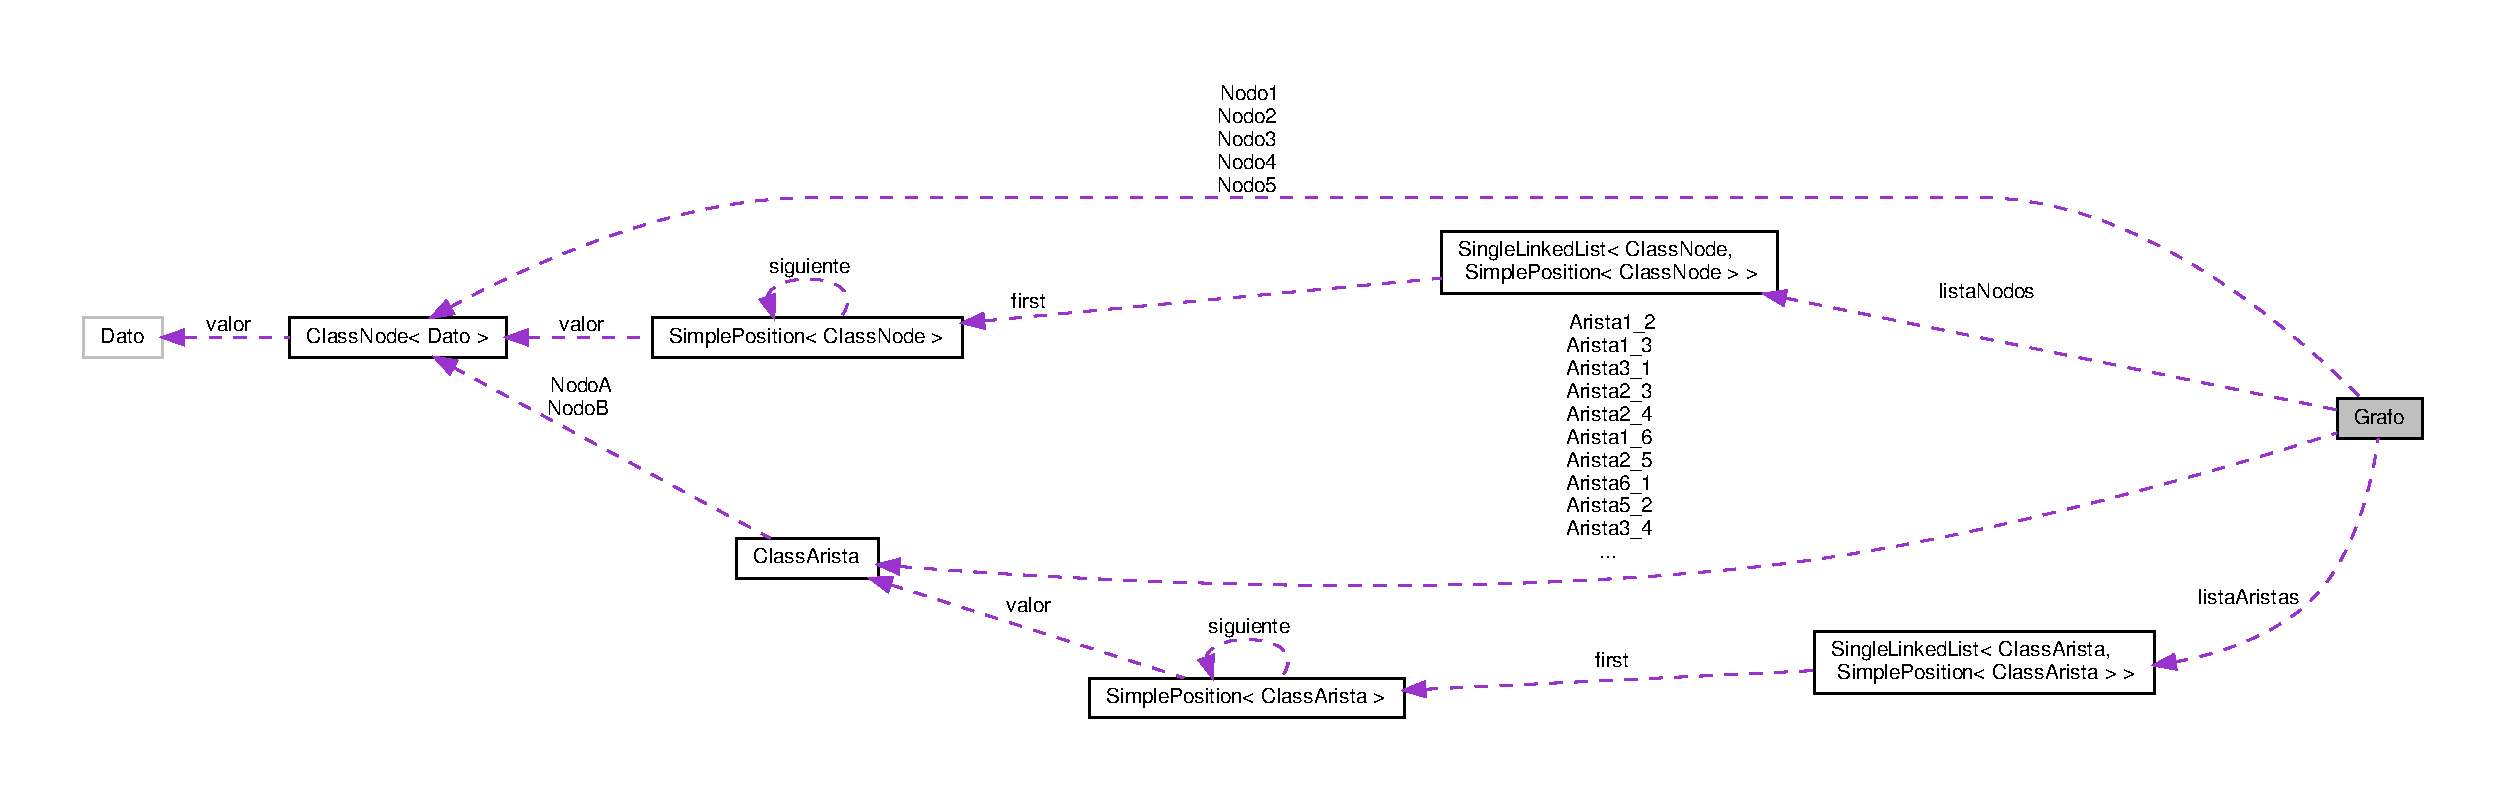
\includegraphics[width=350pt]{class_grafo__coll__graph}
\end{center}
\end{figure}
\subsection*{Public Member Functions}
\begin{DoxyCompactItemize}
\item 
\mbox{\Hypertarget{class_grafo_a371415fb11b7a9f7159071b4f61ef9de}\label{class_grafo_a371415fb11b7a9f7159071b4f61ef9de}} 
void {\bfseries agregar\+Nodo} (int valor, int ID)
\item 
\mbox{\Hypertarget{class_grafo_a43a0d5ad772e6eda6203aad0682ba7a7}\label{class_grafo_a43a0d5ad772e6eda6203aad0682ba7a7}} 
void {\bfseries agregar\+Arista} (int origen, int destino, string ID)
\item 
\mbox{\Hypertarget{class_grafo_a49a0553b340fd2bf7902def48a2e80ce}\label{class_grafo_a49a0553b340fd2bf7902def48a2e80ce}} 
void {\bfseries print\+Nodos} ()
\item 
\mbox{\Hypertarget{class_grafo_a4ff6a98b75185a29e46f135d2f426d9e}\label{class_grafo_a4ff6a98b75185a29e46f135d2f426d9e}} 
void {\bfseries print\+Aristas} ()
\item 
\mbox{\Hypertarget{class_grafo_a7e4e4d7841645b079d7c917a1ada8dd1}\label{class_grafo_a7e4e4d7841645b079d7c917a1ada8dd1}} 
bool {\bfseries hay\+Aristas} (int origen, int destino)
\item 
\mbox{\Hypertarget{class_grafo_ab4c4d98d9eadd6a7c69c0cbcf0bbaa41}\label{class_grafo_ab4c4d98d9eadd6a7c69c0cbcf0bbaa41}} 
int $\ast$$\ast$ {\bfseries matriz\+Adyacencia} ()
\item 
\mbox{\Hypertarget{class_grafo_a1bd0141c8287ecef32e9d8cd360ddc52}\label{class_grafo_a1bd0141c8287ecef32e9d8cd360ddc52}} 
string $\ast$$\ast$ {\bfseries matriz\+Adyacencia\+Texto} ()
\item 
\mbox{\Hypertarget{class_grafo_a1a2bae5ed701b47866ed740d093be38a}\label{class_grafo_a1a2bae5ed701b47866ed740d093be38a}} 
void {\bfseries print\+Matriz} (int $\ast$$\ast$matriz)
\item 
\mbox{\Hypertarget{class_grafo_ad5e0df300d3f4b83623f5787f6b7a2d3}\label{class_grafo_ad5e0df300d3f4b83623f5787f6b7a2d3}} 
void {\bfseries print\+Matriz\+Texto} (string $\ast$$\ast$matriz)
\item 
\mbox{\Hypertarget{class_grafo_aeeff5cd107c3423adbbf3a68818cf4ad}\label{class_grafo_aeeff5cd107c3423adbbf3a68818cf4ad}} 
int {\bfseries a\+Lo\+Ancho} (int origen)
\item 
\mbox{\Hypertarget{class_grafo_a371415fb11b7a9f7159071b4f61ef9de}\label{class_grafo_a371415fb11b7a9f7159071b4f61ef9de}} 
void {\bfseries agregar\+Nodo} (int valor, int ID)
\item 
\mbox{\Hypertarget{class_grafo_a43a0d5ad772e6eda6203aad0682ba7a7}\label{class_grafo_a43a0d5ad772e6eda6203aad0682ba7a7}} 
void {\bfseries agregar\+Arista} (int origen, int destino, string ID)
\item 
\mbox{\Hypertarget{class_grafo_a49a0553b340fd2bf7902def48a2e80ce}\label{class_grafo_a49a0553b340fd2bf7902def48a2e80ce}} 
void {\bfseries print\+Nodos} ()
\item 
\mbox{\Hypertarget{class_grafo_a4ff6a98b75185a29e46f135d2f426d9e}\label{class_grafo_a4ff6a98b75185a29e46f135d2f426d9e}} 
void {\bfseries print\+Aristas} ()
\item 
\mbox{\Hypertarget{class_grafo_a7e4e4d7841645b079d7c917a1ada8dd1}\label{class_grafo_a7e4e4d7841645b079d7c917a1ada8dd1}} 
bool {\bfseries hay\+Aristas} (int origen, int destino)
\item 
\mbox{\Hypertarget{class_grafo_ab4c4d98d9eadd6a7c69c0cbcf0bbaa41}\label{class_grafo_ab4c4d98d9eadd6a7c69c0cbcf0bbaa41}} 
int $\ast$$\ast$ {\bfseries matriz\+Adyacencia} ()
\item 
\mbox{\Hypertarget{class_grafo_a1bd0141c8287ecef32e9d8cd360ddc52}\label{class_grafo_a1bd0141c8287ecef32e9d8cd360ddc52}} 
string $\ast$$\ast$ {\bfseries matriz\+Adyacencia\+Texto} ()
\item 
\mbox{\Hypertarget{class_grafo_a1a2bae5ed701b47866ed740d093be38a}\label{class_grafo_a1a2bae5ed701b47866ed740d093be38a}} 
void {\bfseries print\+Matriz} (int $\ast$$\ast$matriz)
\item 
\mbox{\Hypertarget{class_grafo_ad5e0df300d3f4b83623f5787f6b7a2d3}\label{class_grafo_ad5e0df300d3f4b83623f5787f6b7a2d3}} 
void {\bfseries print\+Matriz\+Texto} (string $\ast$$\ast$matriz)
\item 
\mbox{\Hypertarget{class_grafo_aeeff5cd107c3423adbbf3a68818cf4ad}\label{class_grafo_aeeff5cd107c3423adbbf3a68818cf4ad}} 
int {\bfseries a\+Lo\+Ancho} (int origen)
\end{DoxyCompactItemize}
\subsection*{Public Attributes}
\begin{DoxyCompactItemize}
\item 
\mbox{\Hypertarget{class_grafo_a82bcd52dfaca484b480898965791cd39}\label{class_grafo_a82bcd52dfaca484b480898965791cd39}} 
\hyperlink{class_class_node}{Class\+Node} $\ast$ {\bfseries Nodo1} = new \hyperlink{class_class_node}{Class\+Node}(1, 1)
\item 
\mbox{\Hypertarget{class_grafo_aec40c758df79cb1d44173317edd23e7c}\label{class_grafo_aec40c758df79cb1d44173317edd23e7c}} 
\hyperlink{class_class_node}{Class\+Node} $\ast$ {\bfseries Nodo2} = new \hyperlink{class_class_node}{Class\+Node}(2, 2)
\item 
\mbox{\Hypertarget{class_grafo_a72677ba5c53a48f69421fac847c3484e}\label{class_grafo_a72677ba5c53a48f69421fac847c3484e}} 
\hyperlink{class_class_node}{Class\+Node} $\ast$ {\bfseries Nodo3} = new \hyperlink{class_class_node}{Class\+Node}(3, 3)
\item 
\mbox{\Hypertarget{class_grafo_adbab12f85017195ed784fb59c06141f9}\label{class_grafo_adbab12f85017195ed784fb59c06141f9}} 
\hyperlink{class_class_node}{Class\+Node} $\ast$ {\bfseries Nodo4} = new \hyperlink{class_class_node}{Class\+Node}(4, 4)
\item 
\mbox{\Hypertarget{class_grafo_af17e4f26c857449643855d83c9bcab25}\label{class_grafo_af17e4f26c857449643855d83c9bcab25}} 
\hyperlink{class_class_node}{Class\+Node} $\ast$ {\bfseries Nodo5} = new \hyperlink{class_class_node}{Class\+Node}(5, 5)
\item 
\mbox{\Hypertarget{class_grafo_a4fa6cd6cd1f60b2ea726e1f130af1709}\label{class_grafo_a4fa6cd6cd1f60b2ea726e1f130af1709}} 
\hyperlink{class_class_arista}{Class\+Arista} {\bfseries Arista1\+\_\+2} = \hyperlink{class_class_arista}{Class\+Arista}(Nodo1, Nodo2, \char`\"{}1\+\_\+2\char`\"{})
\item 
\mbox{\Hypertarget{class_grafo_ab021656de1c879b743514b74338e92a0}\label{class_grafo_ab021656de1c879b743514b74338e92a0}} 
\hyperlink{class_class_arista}{Class\+Arista} {\bfseries Arista2\+\_\+3} = \hyperlink{class_class_arista}{Class\+Arista}(Nodo2, Nodo3,\char`\"{}2\+\_\+3\char`\"{})
\item 
\mbox{\Hypertarget{class_grafo_aae6f12f7b29c6771a858a50c4e00f6c0}\label{class_grafo_aae6f12f7b29c6771a858a50c4e00f6c0}} 
\hyperlink{class_class_arista}{Class\+Arista} {\bfseries Arista3\+\_\+4} = \hyperlink{class_class_arista}{Class\+Arista}(Nodo3, Nodo4,\char`\"{}3\+\_\+4\char`\"{})
\item 
\mbox{\Hypertarget{class_grafo_a4c73632cf55dbffd2aacd473dc748bc6}\label{class_grafo_a4c73632cf55dbffd2aacd473dc748bc6}} 
\hyperlink{class_class_arista}{Class\+Arista} {\bfseries Arista4\+\_\+5} = \hyperlink{class_class_arista}{Class\+Arista}(Nodo4, Nodo5,\char`\"{}4\+\_\+5\char`\"{})
\item 
\mbox{\Hypertarget{class_grafo_a4b58976c3b6cc97b9b4ff4fe8193f959}\label{class_grafo_a4b58976c3b6cc97b9b4ff4fe8193f959}} 
\hyperlink{class_class_arista}{Class\+Arista} {\bfseries Arista5\+\_\+2} = \hyperlink{class_class_arista}{Class\+Arista}(Nodo5, Nodo2,\char`\"{}5\+\_\+2\char`\"{})
\item 
\mbox{\Hypertarget{class_grafo_a470b7c92fb2ff9581f4681a7ab4460b4}\label{class_grafo_a470b7c92fb2ff9581f4681a7ab4460b4}} 
\hyperlink{class_class_arista}{Class\+Arista} {\bfseries Arista3\+\_\+1} = \hyperlink{class_class_arista}{Class\+Arista}(Nodo3, Nodo1,\char`\"{}3\+\_\+1\char`\"{})
\item 
\mbox{\Hypertarget{class_grafo_aa9591e6697fbedd3ee5d063c0c7a45fd}\label{class_grafo_aa9591e6697fbedd3ee5d063c0c7a45fd}} 
\hyperlink{class_class_arista}{Class\+Arista} {\bfseries Arista1\+\_\+3} = \hyperlink{class_class_arista}{Class\+Arista}(Nodo1, Nodo3,\char`\"{}1\+\_\+3\char`\"{})
\item 
\mbox{\Hypertarget{class_grafo_ae558a3fd97c12eae5a0741ef8d92823d}\label{class_grafo_ae558a3fd97c12eae5a0741ef8d92823d}} 
\hyperlink{class_class_arista}{Class\+Arista} {\bfseries Arista2\+\_\+4} = \hyperlink{class_class_arista}{Class\+Arista}(Nodo2, Nodo4,\char`\"{}2\+\_\+4\char`\"{})
\item 
\mbox{\Hypertarget{class_grafo_abe8c209f3afee993d458ea5e607a5d09}\label{class_grafo_abe8c209f3afee993d458ea5e607a5d09}} 
\hyperlink{class_class_arista}{Class\+Arista} {\bfseries Arista2\+\_\+5} = \hyperlink{class_class_arista}{Class\+Arista}(Nodo2, Nodo5,\char`\"{}2\+\_\+5\char`\"{})
\item 
\mbox{\Hypertarget{class_grafo_a48094bc6d22cacab54e80d75c9df517a}\label{class_grafo_a48094bc6d22cacab54e80d75c9df517a}} 
\hyperlink{class_class_arista}{Class\+Arista} {\bfseries Arista5\+\_\+6} = \hyperlink{class_class_arista}{Class\+Arista}(Nodo5, Nodo6,\char`\"{}5\+\_\+6\char`\"{})
\item 
\mbox{\Hypertarget{class_grafo_af3b5ec1e719de72a0c6ddad7c03a85b7}\label{class_grafo_af3b5ec1e719de72a0c6ddad7c03a85b7}} 
\hyperlink{class_class_arista}{Class\+Arista} {\bfseries Arista1\+\_\+6} = \hyperlink{class_class_arista}{Class\+Arista}(Nodo1, Nodo6,\char`\"{}1\+\_\+6\char`\"{})
\item 
\mbox{\Hypertarget{class_grafo_ab29129c53c7912aa1bbd603b32d7b2d3}\label{class_grafo_ab29129c53c7912aa1bbd603b32d7b2d3}} 
\hyperlink{class_class_arista}{Class\+Arista} {\bfseries Arista3\+\_\+6} = \hyperlink{class_class_arista}{Class\+Arista}(Nodo3, Nodo6,\char`\"{}3\+\_\+6\char`\"{})
\item 
\mbox{\Hypertarget{class_grafo_a00b2a3cb2e962106be5cbcf60ce668de}\label{class_grafo_a00b2a3cb2e962106be5cbcf60ce668de}} 
\hyperlink{class_class_arista}{Class\+Arista} {\bfseries Arista6\+\_\+1} = \hyperlink{class_class_arista}{Class\+Arista}(Nodo6, Nodo1,\char`\"{}6\+\_\+1\char`\"{})
\item 
\mbox{\Hypertarget{class_grafo_a5092860f200f0c1e2fb8bf0f871f9827}\label{class_grafo_a5092860f200f0c1e2fb8bf0f871f9827}} 
\hyperlink{class_single_linked_list}{Single\+Linked\+List}$<$ \hyperlink{class_class_node}{Class\+Node}, \hyperlink{class_simple_position}{Simple\+Position}$<$ \hyperlink{class_class_node}{Class\+Node} $>$ $>$ {\bfseries lista\+Nodos}
\item 
\mbox{\Hypertarget{class_grafo_ad8576a589d4c74776091518f40943b9c}\label{class_grafo_ad8576a589d4c74776091518f40943b9c}} 
\hyperlink{class_single_linked_list}{Single\+Linked\+List}$<$ \hyperlink{class_class_arista}{Class\+Arista}, \hyperlink{class_simple_position}{Simple\+Position}$<$ \hyperlink{class_class_arista}{Class\+Arista} $>$ $>$ {\bfseries lista\+Aristas}
\item 
\mbox{\Hypertarget{class_grafo_acba59ba1597a3602b716baf94ee1489b}\label{class_grafo_acba59ba1597a3602b716baf94ee1489b}} 
int {\bfseries contador\+Nodos} = 0
\item 
\mbox{\Hypertarget{class_grafo_a89bdc2737171d2381341cfa227cb4029}\label{class_grafo_a89bdc2737171d2381341cfa227cb4029}} 
int {\bfseries contador\+Aristas} = 0
\end{DoxyCompactItemize}


\subsection{Detailed Description}


Definition at line 26 of file graph.\+h.



The documentation for this class was generated from the following files\+:\begin{DoxyCompactItemize}
\item 
Algoritmos\+De\+Terceros/include/graph.\+h\item 
Algoritmos\+De\+Terceros/include/graph2.\+h\item 
Algoritmos\+De\+Terceros/include/Mi\+Clase\+Grafo.\+h\end{DoxyCompactItemize}

\hypertarget{class_graph}{}\section{Graph Class Reference}
\label{class_graph}\index{Graph@{Graph}}
\subsection*{Public Member Functions}
\begin{DoxyCompactItemize}
\item 
\mbox{\Hypertarget{class_graph_af3ff6b295df8bf3bee0bafd7c7d56915}\label{class_graph_af3ff6b295df8bf3bee0bafd7c7d56915}} 
{\bfseries Graph} (int V)
\item 
\mbox{\Hypertarget{class_graph_a6e0b786e5023445457b8c742f5f15cf2}\label{class_graph_a6e0b786e5023445457b8c742f5f15cf2}} 
void {\bfseries Add\+Weighted\+Edge} (int u, int v, int w)
\item 
\mbox{\Hypertarget{class_graph_a7d345850bf222bc15f9d2a364d628bf7}\label{class_graph_a7d345850bf222bc15f9d2a364d628bf7}} 
int {\bfseries find\+\_\+set} (int i)
\item 
\mbox{\Hypertarget{class_graph_ac17601621203f1782504e6c6e3bf612a}\label{class_graph_ac17601621203f1782504e6c6e3bf612a}} 
void {\bfseries union\+\_\+set} (int u, int v)
\item 
\mbox{\Hypertarget{class_graph_a1de36bcb031663da79fc00f5aa0eaede}\label{class_graph_a1de36bcb031663da79fc00f5aa0eaede}} 
void {\bfseries kruskal} ()
\item 
\mbox{\Hypertarget{class_graph_a2ecf3dd3c4897aa924da8e5c221a8509}\label{class_graph_a2ecf3dd3c4897aa924da8e5c221a8509}} 
void {\bfseries print} ()
\item 
\mbox{\Hypertarget{class_graph_af3ff6b295df8bf3bee0bafd7c7d56915}\label{class_graph_af3ff6b295df8bf3bee0bafd7c7d56915}} 
{\bfseries Graph} (int V)
\item 
\mbox{\Hypertarget{class_graph_a6e0b786e5023445457b8c742f5f15cf2}\label{class_graph_a6e0b786e5023445457b8c742f5f15cf2}} 
void {\bfseries Add\+Weighted\+Edge} (int u, int v, int w)
\item 
\mbox{\Hypertarget{class_graph_a7d345850bf222bc15f9d2a364d628bf7}\label{class_graph_a7d345850bf222bc15f9d2a364d628bf7}} 
int {\bfseries find\+\_\+set} (int i)
\item 
\mbox{\Hypertarget{class_graph_ac17601621203f1782504e6c6e3bf612a}\label{class_graph_ac17601621203f1782504e6c6e3bf612a}} 
void {\bfseries union\+\_\+set} (int u, int v)
\item 
\mbox{\Hypertarget{class_graph_a1de36bcb031663da79fc00f5aa0eaede}\label{class_graph_a1de36bcb031663da79fc00f5aa0eaede}} 
void {\bfseries kruskal} ()
\item 
\mbox{\Hypertarget{class_graph_a2ecf3dd3c4897aa924da8e5c221a8509}\label{class_graph_a2ecf3dd3c4897aa924da8e5c221a8509}} 
void {\bfseries print} ()
\end{DoxyCompactItemize}


\subsection{Detailed Description}


Definition at line 17 of file main.\+cpp.



The documentation for this class was generated from the following files\+:\begin{DoxyCompactItemize}
\item 
Algoritmos\+De\+Terceros/main.\+cpp\item 
Algoritmos\+De\+Terceros/main\+Krus.\+cpp\end{DoxyCompactItemize}

\hypertarget{class_queue}{}\section{Queue$<$ D $>$ Class Template Reference}
\label{class_queue}\index{Queue$<$ D $>$@{Queue$<$ D $>$}}
\subsection*{Public Member Functions}
\begin{DoxyCompactItemize}
\item 
\mbox{\Hypertarget{class_queue_a24f783b719e19d65b3ee5a98b6daee3a}\label{class_queue_a24f783b719e19d65b3ee5a98b6daee3a}} 
{\bfseries Queue} (const \hyperlink{class_queue}{Queue} \&orig)
\item 
\mbox{\Hypertarget{class_queue_a80e37c5fc154e7a3788b6b25bb7399b8}\label{class_queue_a80e37c5fc154e7a3788b6b25bb7399b8}} 
void {\bfseries enqueue} (D d)
\item 
\mbox{\Hypertarget{class_queue_ae3a41c4439bb5914acce8ef329a05512}\label{class_queue_ae3a41c4439bb5914acce8ef329a05512}} 
D {\bfseries dequeue} ()
\item 
\mbox{\Hypertarget{class_queue_a24f783b719e19d65b3ee5a98b6daee3a}\label{class_queue_a24f783b719e19d65b3ee5a98b6daee3a}} 
{\bfseries Queue} (const \hyperlink{class_queue}{Queue} \&orig)
\item 
\mbox{\Hypertarget{class_queue_a80e37c5fc154e7a3788b6b25bb7399b8}\label{class_queue_a80e37c5fc154e7a3788b6b25bb7399b8}} 
void {\bfseries enqueue} (D d)
\item 
\mbox{\Hypertarget{class_queue_ae3a41c4439bb5914acce8ef329a05512}\label{class_queue_ae3a41c4439bb5914acce8ef329a05512}} 
D {\bfseries dequeue} ()
\end{DoxyCompactItemize}


\subsection{Detailed Description}
\subsubsection*{template$<$typename D$>$\newline
class Queue$<$ D $>$}



Definition at line 6 of file Queue.\+h.



The documentation for this class was generated from the following file\+:\begin{DoxyCompactItemize}
\item 
Algoritmos\+De\+Terceros/include/pilas\+Colas/Queue.\+h\end{DoxyCompactItemize}

\hypertarget{class_simple_position}{}\section{Simple\+Position$<$ Dato $>$ Class Template Reference}
\label{class_simple_position}\index{Simple\+Position$<$ Dato $>$@{Simple\+Position$<$ Dato $>$}}
\subsection*{Public Member Functions}
\begin{DoxyCompactItemize}
\item 
\mbox{\Hypertarget{class_simple_position_a6b6e102942c3cf1797735255897402b5}\label{class_simple_position_a6b6e102942c3cf1797735255897402b5}} 
{\bfseries Simple\+Position} (Dato $\ast$valor)
\end{DoxyCompactItemize}
\subsection*{Public Attributes}
\begin{DoxyCompactItemize}
\item 
\mbox{\Hypertarget{class_simple_position_a65bb8d8c8a3011fb28ea1a324c7910dc}\label{class_simple_position_a65bb8d8c8a3011fb28ea1a324c7910dc}} 
\hyperlink{class_simple_position}{Simple\+Position}$<$ Dato $>$ $\ast$ {\bfseries siguiente} = 0x0
\item 
\mbox{\Hypertarget{class_simple_position_adfc8434ef460d5c20d71494ad6a48c52}\label{class_simple_position_adfc8434ef460d5c20d71494ad6a48c52}} 
Dato $\ast$ {\bfseries valor}
\end{DoxyCompactItemize}


\subsection{Detailed Description}
\subsubsection*{template$<$typename Dato$>$\newline
class Simple\+Position$<$ Dato $>$}



Definition at line 8 of file Simple\+Position.\+h.



The documentation for this class was generated from the following file\+:\begin{DoxyCompactItemize}
\item 
/home/jzunigame/\+Documentos/\+A\+\_\+\+Algoritmos/\+A\+\_\+\+Git/\+Laboratorios/\+Lab4 Listas/include/Simple\+Position.\+h\end{DoxyCompactItemize}

\hypertarget{class_single_linked_list}{}\section{Single\+Linked\+List$<$ Element, Single\+Position $>$ Class Template Reference}
\label{class_single_linked_list}\index{Single\+Linked\+List$<$ Element, Single\+Position $>$@{Single\+Linked\+List$<$ Element, Single\+Position $>$}}


Collaboration diagram for Single\+Linked\+List$<$ Element, Single\+Position $>$\+:
\nopagebreak
\begin{figure}[H]
\begin{center}
\leavevmode
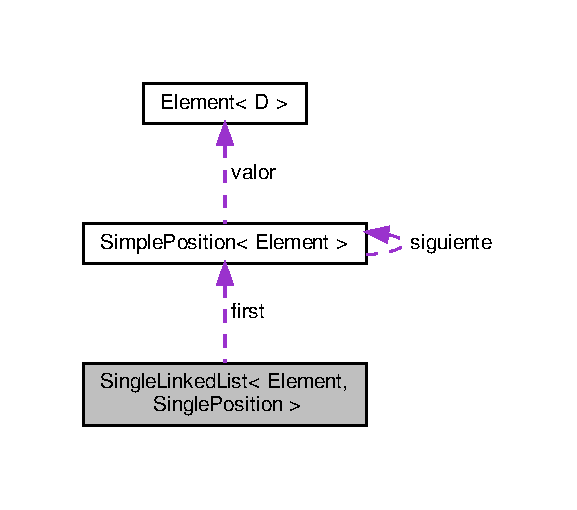
\includegraphics[width=277pt]{class_single_linked_list__coll__graph}
\end{center}
\end{figure}
\subsection*{Public Member Functions}
\begin{DoxyCompactItemize}
\item 
\mbox{\Hypertarget{class_single_linked_list_aa94809f2f418d8ae0800c07ad2d3ed94}\label{class_single_linked_list_aa94809f2f418d8ae0800c07ad2d3ed94}} 
Single\+Position \& {\bfseries insert} (const \hyperlink{class_element}{Element} \&dato)
\item 
\mbox{\Hypertarget{class_single_linked_list_a22c895b2d3effcce5983b991a380027b}\label{class_single_linked_list_a22c895b2d3effcce5983b991a380027b}} 
\hyperlink{class_element}{Element} $\ast$ {\bfseries get\+Direccion} (int elemento)
\item 
\mbox{\Hypertarget{class_single_linked_list_a64d9f3e1bad3eec787d2bcc7255c1311}\label{class_single_linked_list_a64d9f3e1bad3eec787d2bcc7255c1311}} 
void \hyperlink{class_single_linked_list_a64d9f3e1bad3eec787d2bcc7255c1311}{print} ()
\begin{DoxyCompactList}\small\item\em Funcion que imprime los datos de la lista. \end{DoxyCompactList}\item 
\mbox{\Hypertarget{class_single_linked_list_a09b8d66c2be112326210373514f32cd7}\label{class_single_linked_list_a09b8d66c2be112326210373514f32cd7}} 
Single\+Position $\ast$ {\bfseries devolver\+Posicion} (int item)
\item 
\mbox{\Hypertarget{class_single_linked_list_aebc417269f785f2f8d3689403e7a6524}\label{class_single_linked_list_aebc417269f785f2f8d3689403e7a6524}} 
bool {\bfseries verificar} (\hyperlink{class_class_node}{Class\+Node} $\ast$origen, \hyperlink{class_class_node}{Class\+Node} $\ast$destino)
\item 
\mbox{\Hypertarget{class_single_linked_list_a2ed18090fd23eba38a668e40e0bca2c4}\label{class_single_linked_list_a2ed18090fd23eba38a668e40e0bca2c4}} 
Single\+Position $\ast$ {\bfseries devolver\+Posicion\+Desde\+Valor} (int valor)
\item 
\mbox{\Hypertarget{class_single_linked_list_aa94809f2f418d8ae0800c07ad2d3ed94}\label{class_single_linked_list_aa94809f2f418d8ae0800c07ad2d3ed94}} 
Single\+Position \& {\bfseries insert} (const \hyperlink{class_element}{Element} \&dato)
\item 
\mbox{\Hypertarget{class_single_linked_list_a22c895b2d3effcce5983b991a380027b}\label{class_single_linked_list_a22c895b2d3effcce5983b991a380027b}} 
\hyperlink{class_element}{Element} $\ast$ {\bfseries get\+Direccion} (int elemento)
\item 
\mbox{\Hypertarget{class_single_linked_list_a64d9f3e1bad3eec787d2bcc7255c1311}\label{class_single_linked_list_a64d9f3e1bad3eec787d2bcc7255c1311}} 
void \hyperlink{class_single_linked_list_a64d9f3e1bad3eec787d2bcc7255c1311}{print} ()
\begin{DoxyCompactList}\small\item\em Funcion que imprime los datos de la lista. \end{DoxyCompactList}\item 
\mbox{\Hypertarget{class_single_linked_list_a09b8d66c2be112326210373514f32cd7}\label{class_single_linked_list_a09b8d66c2be112326210373514f32cd7}} 
Single\+Position $\ast$ {\bfseries devolver\+Posicion} (int item)
\item 
\mbox{\Hypertarget{class_single_linked_list_aebc417269f785f2f8d3689403e7a6524}\label{class_single_linked_list_aebc417269f785f2f8d3689403e7a6524}} 
bool {\bfseries verificar} (\hyperlink{class_class_node}{Class\+Node} $\ast$origen, \hyperlink{class_class_node}{Class\+Node} $\ast$destino)
\item 
\mbox{\Hypertarget{class_single_linked_list_a2ed18090fd23eba38a668e40e0bca2c4}\label{class_single_linked_list_a2ed18090fd23eba38a668e40e0bca2c4}} 
Single\+Position $\ast$ {\bfseries devolver\+Posicion\+Desde\+Valor} (int valor)
\end{DoxyCompactItemize}
\subsection*{Public Attributes}
\begin{DoxyCompactItemize}
\item 
\mbox{\Hypertarget{class_single_linked_list_a870bf08579b5a9cb4d570b57cbcdc826}\label{class_single_linked_list_a870bf08579b5a9cb4d570b57cbcdc826}} 
\hyperlink{class_simple_position}{Simple\+Position}$<$ \hyperlink{class_element}{Element} $>$ $\ast$ {\bfseries first}
\item 
\mbox{\Hypertarget{class_single_linked_list_a8449fa747af940f9d1c9c6e8758539b8}\label{class_single_linked_list_a8449fa747af940f9d1c9c6e8758539b8}} 
int {\bfseries items} =0
\end{DoxyCompactItemize}


\subsection{Detailed Description}
\subsubsection*{template$<$typename Element, typename Single\+Position$>$\newline
class Single\+Linked\+List$<$ Element, Single\+Position $>$}



Definition at line 9 of file Single\+Linked\+List.\+h.



The documentation for this class was generated from the following file\+:\begin{DoxyCompactItemize}
\item 
Algoritmos\+De\+Terceros/include/\+Listas/Single\+Linked\+List.\+h\end{DoxyCompactItemize}

\hypertarget{class_stack}{}\section{Stack$<$ D $>$ Class Template Reference}
\label{class_stack}\index{Stack$<$ D $>$@{Stack$<$ D $>$}}
\subsection*{Public Member Functions}
\begin{DoxyCompactItemize}
\item 
\mbox{\Hypertarget{class_stack_a55e5793404d42ba905f1a7ab90092807}\label{class_stack_a55e5793404d42ba905f1a7ab90092807}} 
{\bfseries Stack} (const \hyperlink{class_stack}{Stack} \&orig)
\item 
\mbox{\Hypertarget{class_stack_acf4211784a34b61ed4ba49272f23351f}\label{class_stack_acf4211784a34b61ed4ba49272f23351f}} 
void {\bfseries push} (D d)
\item 
\mbox{\Hypertarget{class_stack_a54e8fd6fd2a8b828b7b66f171499e956}\label{class_stack_a54e8fd6fd2a8b828b7b66f171499e956}} 
D {\bfseries pop} ()
\item 
\mbox{\Hypertarget{class_stack_a5717795349538863baaeafe7e25df76a}\label{class_stack_a5717795349538863baaeafe7e25df76a}} 
D {\bfseries peek} ()
\end{DoxyCompactItemize}


\subsection{Detailed Description}
\subsubsection*{template$<$typename D$>$\newline
class Stack$<$ D $>$}



Definition at line 6 of file Stack.\+h.



The documentation for this class was generated from the following file\+:\begin{DoxyCompactItemize}
\item 
Includes/Stack.\+h\end{DoxyCompactItemize}

%--- End generated contents ---

% Index
\backmatter
\newpage
\phantomsection
\clearemptydoublepage
\addcontentsline{toc}{chapter}{Index}
\printindex

\end{document}
